\documentclass[12pt, a4paper, oneside]{ctexart}
\usepackage{amsmath, amsthm, amssymb, graphicx,fancyhdr,geometry , subfigure,verbatim}
\usepackage[bookmarks=true, colorlinks, citecolor=blue, linkcolor=black]{hyperref}
\geometry{a4paper,scale=0.75}
\pagestyle{fancy}
\fancyhf{} % Clear all headers and footers
\fancyhead[L]{运筹学作业}
\fancyhead[C]{} % Center header - document title
\fancyhead[R]{王德茂} % Right header - page number
\fancyfoot[C]{\thepage}

\begin{document}
\section*{问题提出}
敌对的两个国家都面临着两种选择:扩充军备或裁减军备:如果双方进行军备竞赛(扩军),都将为此付出3000亿美元的代价;如果双方都裁军,则可以省下这
笔钱.但是倘若有一方裁军,另一方扩军,则扩军一方发动侵略战争,占领对方领土,从而可获益1万亿美元.裁军一方由于军事失败而又丧失国土则可以认为损失
无限,试建立该问题的对策模型,并求该问题的纳什平衡解.

\section*{建立模型}
这是一个典型的博弈论问题,可以通过构建一个矩阵博弈来求解。

假设两个国家为 A 和 B,各自的策略为扩充军备或裁减军备。我们将两个国家的收益用矩阵表示出来。

收益矩阵如下:

\begin{itemize}
    \item 如果双方都选择扩充军备 (E),双方都损失 3000 亿美元。
    \item 如果双方都选择裁减军备 (C),双方都节省 3000 亿美元。
    \item 如果一方扩充军备,另一方裁减军备,扩充军备的一方获得 1 万亿美元,而裁减军备的一方损失无限。
\end{itemize}

\[
\begin{array}{c|c|c}
    & \text{B 选择扩军 (E)} & \text{B 选择裁军 (C)} \\
    \hline
    \text{A 选择扩军 (E)} & (-3000, -3000) & (10000, -\infty) \\
    \hline
    \text{A 选择裁军 (C)} & (-\infty, 10000) & (3000, 3000) \\
\end{array}
\]
我们使用LINGO编程求解该双矩阵对策问题。
\section*{代码实现}
\begin{verbatim}
    MAX =  -6*x1*y1 -990 *x1*y2  -990 * x2 *y1 +6 *x2*y2 - v1 - v2;
    -3*x1 + 10*x2 <= v1;
    -1000*x1 + 3*x2<= v1;
    -3*y1 + 10*y2 <= v2;
    -1000*y1 + 3*y2 <= v2;
    x1<=1;
    x2<=1;
    y1<=1;
    y2<=1;
    x1+x2=1;
    y1+y2=1;
    @gin(x1);
    @gin(x2);
    @gin(y1);
    @gin(y2);
\end{verbatim}

\begin{figure}[htbp]
    \centering
    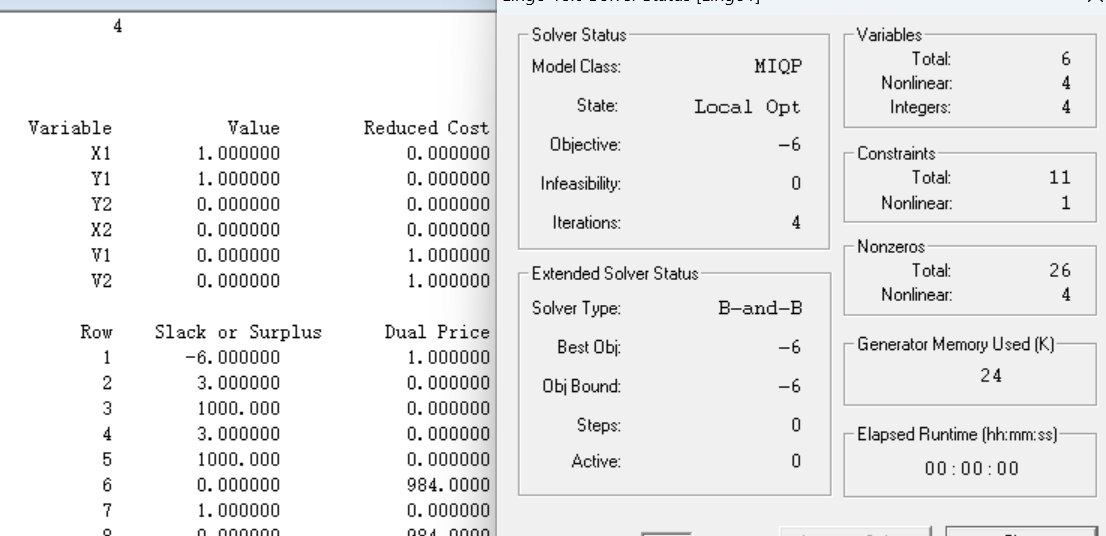
\includegraphics[scale = 0.4]{image.png}
    \caption{求解结果}
\end{figure} 
\section*{结论}
通过上述博弈模型和代码计算,纳什均衡是双方都选择扩充军备。这是因为在任何一方裁减军备的情况下,另一方扩充军备会导致裁军方损失无限,而扩军方获益巨大。因此,为避免无限损失,双方都会选择扩军,即使会付出3000亿美元的代价。
\end{document} 
